\section{隐式微分}
\label{sec:bilevel-implicit}

在定理~\ref{thm:bilevel-local-branch}成立的分支上，怎样计算外层目标的导数？关键的观察是，求导只需要当前解点处的局部关系。至于这个解是怎样迭代得到的，算法走过了多少步，都不进入公式，也不必保存。

\subsection{超梯度}
\label{sec:bilevel-hypergradient}

设$\hat{\bm{y}}(\bm{x})$是所追踪的分支，外层目标为$\Phi(\bm{x})=F(\bm{x},\hat{\bm{y}}(\bm{x}))$。若内解唯一且满足定理~\ref{thm:bilevel-strong-convex-map}，这条分支就是$\bm{y}^\star(\bm{x})$。$\Phi$对$\bm{x}$的梯度称为\termalias{超梯度-hypergradient}{超梯度}（hypergradient）。“超”在这里指外层，与第~\ref{chap:penalty-multiplier-methods}章凹函数的超梯度（supergradient）是两回事。

\paragraph{主要思想：把响应接到外层}
由链式法则，$\Phi$的梯度由两部分组成：
\[
 \nabla\Phi=\nabla_{\bm{x}}F+\bm{D}^{\top}\nabla_{\bm{y}}F.
\]
第一项是直接作用，第二项是响应。把式~\eqref{eq:bilevel-branch-derivative}代入第二项，并利用$\bm{H}$对称，得到
\[
 \bm{D}^{\top}\nabla_{\bm{y}}F=-\bm{B}^{\top}\bm{H}^{-1}\nabla_{\bm{y}}F.
\]

这个式子不必先算出$\bm{H}^{-1}\bm{B}$这个$d\times n$矩阵。先解一个以$\nabla_{\bm{y}}F$为右端的方程，得到的向量再乘$\bm{B}^{\top}$即可。

\begin{theorem}[隐式超梯度]
\label{thm:bilevel-hypergradient}
设定理~\ref{thm:bilevel-local-branch}的条件成立，$F$在$(\bm{x}_0,\bm{y}_0)$附近连续可微。则$\Phi(\bm{x})=F(\bm{x},\hat{\bm{y}}(\bm{x}))$连续可微，且
\begin{equation}
 \nabla\Phi=\nabla_{\bm{x}}F-\bm{B}^{\top}\bm{v},
 \qquad\bm{H}\bm{v}=\nabla_{\bm{y}}F,
 \label{eq:bilevel-hypergradient}
\end{equation}
其中所有导数都在$(\bm{x},\hat{\bm{y}}(\bm{x}))$处取值。
\end{theorem}

\begin{proof}
$\hat{\bm{y}}$连续可微，$F$连续可微，由链式法则$\Phi$连续可微，其梯度是上面的两项之和。$\bm{H}$正定，所以方程$\bm{H}\bm{v}=\nabla_{\bm{y}}F$有唯一解，即$\bm{v}=\bm{H}^{-1}\nabla_{\bm{y}}F$，代入即得式~\eqref{eq:bilevel-hypergradient}。
\end{proof}

式~\eqref{eq:bilevel-hypergradient}中的$\bm{H}\bm{v}=\nabla_{\bm{y}}F$称为\term{伴随方程}（adjoint equation）。用这种方法求超梯度的做法称为\term{隐式微分}（implicit differentiation），因为内解没有显式公式，导数是从定义它的方程中得出的。

\paragraph{$\bm{v}$是内层梯度的价格}
$\bm{v}$有一个直接的含义。设想把驻点方程改成$\nabla_{\bm{y}}g=\bm{\varepsilon}$，也就是给内层梯度一点小扰动。内解移动$\bm{H}^{-1}\bm{\varepsilon}$，外层值变化约为
\[
 \langle\nabla_{\bm{y}}F,\bm{H}^{-1}\bm{\varepsilon}\rangle=\langle\bm{v},\bm{\varepsilon}\rangle.
\]
所以$\bm{v}$是内层梯度每单位扰动在外层的价格，含义和约束乘子作为影子价格相同。

$\bm{x}$改变$\Delta\bm{x}$时，内层梯度在原来的解点偏移$\bm{B}\Delta\bm{x}$，内解要把这份偏移抵消掉，相当于对内层施加了$-\bm{B}\Delta\bm{x}$的扰动。价格乘以扰动量，就得到响应项$-\langle\bm{B}^{\top}\bm{v},\Delta\bm{x}\rangle$。这个价格只在一阶范围内有效，$\Delta\bm{x}$大了或分支切换了，它就不再准确。

图~\ref{fig:bilevel-adjoint-chain}把这条因果链画了出来。上面一行顺着原因往下算，要带着$n$个方向的$\Delta\bm{x}$走完全程。下面一行从外层往回算，只带一个向量。标量外层目标、很多外层变量时，后者便宜得多。

\begin{BookInlineFigure}
 \centering
 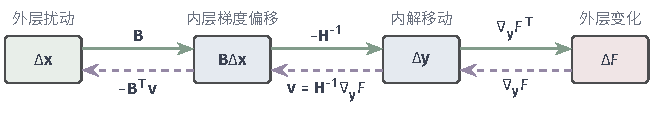
\includegraphics[width=110.6mm]{figures/05-optimization/07-multiple-criteria-and-nested-optimization/tikz/bilevel-adjoint-chain/figure.pdf}
 \caption{超梯度的因果链。绿色实线从外层扰动算到外层变化，每个方向$\Delta\bm{x}$算一次。紫色虚线从外层梯度往回算，一次得到全部分量的梯度，$\bm{v}$是内层梯度偏移的价格。}
 \label{fig:bilevel-adjoint-chain}
\end{BookInlineFigure}

\paragraph{手算核对}
对正则拟合例~\eqref{eq:bilevel-ridge}，在$x=1$处，各量为
\[
 y^\star=\frac32,\qquad H=1+x=2,\qquad B=y^\star=\frac32,\qquad\partial_yF=y^\star-1=\frac12.
\]

解伴随方程，得到
\[
 v=\frac{\partial_yF}{H}=\frac14.
\]

$F$不含$x$，所以由式~\eqref{eq:bilevel-hypergradient}，
\[
 \Phi'(1)=0-Bv=-\frac38.
\]

直接对$\Phi$求导来核对。由链式法则，
\[
 \Phi'(x)=(y^\star-1)\,\frac{\mathrm{d}y^\star}{\mathrm{d}x},
\]
在$x=1$处等于$\frac12\times(-\frac34)=-\frac38$，两者相同。同样可算出$\Phi'(0)=-6$；在$x=2$处$\partial_yF=0$，$v=0$，$\Phi'(2)=0$，这正是最小点。

\paragraph{第二项不能丢}
这个例子里$\nabla_{\bm{x}}F=0$。如果只对$F$求偏导，也就是把$y$固定住，得到的斜率处处是$0$，结论将是$x$不用调整。图~\ref{fig:bilevel-hypergrad-tangent}比较了这两条线。忽略响应项，求的是“固定内解时的偏导数”，并不是双层目标的导数。

\begin{BookInlineFigure}
 \centering
 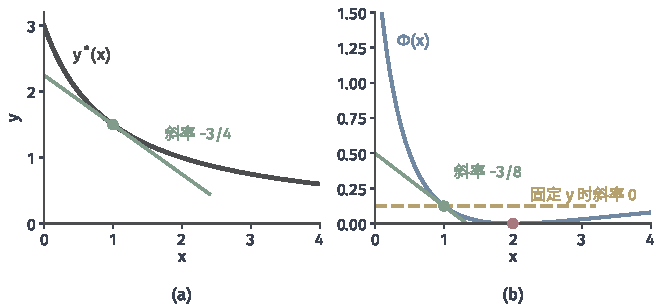
\includegraphics[width=112mm]{figures/05-optimization/07-multiple-criteria-and-nested-optimization/matplotlib/bilevel-hypergrad-tangent/figure.pdf}
 \caption{正则拟合例中$x=1$处的导数。(a)内解曲线的切线，斜率是$\mathrm{d}y^\star/\mathrm{d}x=-3/4$。(b)$\Phi$的切线（绿）斜率是超梯度$-3/8$；黄色虚线是把$y$固定在$y^\star(1)$时的外层函数，斜率为$0$。红点是$\Phi$的最小点。}
 \label{fig:bilevel-hypergrad-tangent}
\end{BookInlineFigure}

\paragraph{与极小极大的联系}
式~\eqref{eq:bilevel-hypergradient}也说明了表~\ref{tab:bilevel-vs-minimax}的最后一行。若$F=-g$，内解处$\nabla_{\bm{y}}F=-\nabla_{\bm{y}}g=\bm{0}$，于是$\bm{v}=\bm{0}$，超梯度退化为$\nabla_{\bm{x}}F$。内解的移动对外层值只有二阶影响，这就是第~\ref{chap:minimax-optimization}章和第~\ref{chap:parametric-sensitivity}章的包络关系。一般的双层问题没有这种抵消，响应项必须计算。

\subsection{线性方程求解}
\label{sec:bilevel-linear-solve}

$d$很大时$\bm{H}$存不下，更不用说求逆。本小节要解决的问题是：怎样只用$\bm{H}$与向量的乘积解伴随方程，以及这个方程解得不准会造成多大的超梯度误差。

\paragraph{主要思想：只用矩阵—向量积}
解$\bm{H}\bm{v}=\nabla_{\bm{y}}F$的迭代法只需要反复计算$\bm{H}\bm{u}$。这个乘积不需要$\bm{H}$的元素，它是内层梯度沿$\bm{u}$方向的方向导数：
\begin{equation}
 \bm{H}\bm{u}=\frac{\mathrm{d}}{\mathrm{d}s}\nabla_{\bm{y}}g(\bm{x},\bm{y}+s\bm{u})\Big|_{s=0}.
 \label{eq:bilevel-hvp}
\end{equation}

这称为\term{Hessian向量积}（Hessian-vector product）。用自动求导时，它的代价是梯度计算的常数倍，也可以用内层梯度的差分近似。$\bm{B}^{\top}\bm{v}$同样如此，它是标量$\langle\nabla_{\bm{y}}g,\bm{v}\rangle$（固定$\bm{v}$）对$\bm{x}$的梯度。

$\bm{H}$对称正定时，共轭梯度法是自然的选择，算法的推导可参考\BookChapterRef{chap:krylov-methods}{卷二第15章“Krylov子空间法”}。第~$k$步用到的量都按下面的递推得到，$\alpha^{(k)}$和$\beta^{(k)}$在本小节里表示共轭梯度法自己的系数：
\begin{equation}
 \begin{gathered}
 \alpha^{(k)}=\frac{\lVert\bm{r}^{(k)}\rVert_2^2}{\langle\bm{d}^{(k)},\bm{H}\bm{d}^{(k)}\rangle},\qquad
 \bm{v}^{(k+1)}=\bm{v}^{(k)}+\alpha^{(k)}\bm{d}^{(k)},\\
 \bm{r}^{(k+1)}=\bm{r}^{(k)}-\alpha^{(k)}\bm{H}\bm{d}^{(k)},\\
 \beta^{(k)}=\frac{\lVert\bm{r}^{(k+1)}\rVert_2^2}{\lVert\bm{r}^{(k)}\rVert_2^2},\qquad
 \bm{d}^{(k+1)}=\bm{r}^{(k+1)}+\beta^{(k)}\bm{d}^{(k)}.
 \end{gathered}
 \label{eq:bilevel-cg}
\end{equation}

\paragraph{计算过程}
下面用二维内层走一遍全过程。内层是带二次惩罚的最小二乘，外层把结果和目标点比较：
\[
 g(x,\bm{y})=\frac12\lVert\bm{A}\bm{y}-\bm{b}\rVert_2^2+\frac{x}{2}\lVert\bm{y}\rVert_2^2,\qquad F(\bm{y})=\frac12\lVert\bm{y}-\bm{c}\rVert_2^2.
\]

数据取为
\[
 \bm{A}=\begin{bmatrix}1&1\\0&1\end{bmatrix},\qquad
 \bm{b}=\begin{bmatrix}3\\1\end{bmatrix},\qquad
 \bm{c}=\begin{bmatrix}0\\2\end{bmatrix}.
\]

\needspace{6\baselineskip}
\paragraph{变量}
\begin{itemize}
 \item 内解$\bm{y}\in\mathbb{R}^d$，事先由内层算法得到。
 \item 伴随向量的迭代值$\bm{v}^{(k)}\in\mathbb{R}^d$，残差$\bm{r}^{(k)}=\nabla_{\bm{y}}F-\bm{H}\bm{v}^{(k)}$，搜索方向$\bm{d}^{(k)}\in\mathbb{R}^d$。
 \item 超梯度估计$\hat{\bm{\gamma}}^{(k)}\in\mathbb{R}^n$，把式~\eqref{eq:bilevel-hypergradient}中的$\bm{v}$换成$\bm{v}^{(k)}$得到。
\end{itemize}

\paragraph{初始化}
先在当前$\bm{x}$处得到内解，计算外层梯度，并置$\bm{v}^{(0)}=\bm{0}$，$\bm{r}^{(0)}=\bm{d}^{(0)}=\nabla_{\bm{y}}F$。

例中取$x=1$。$\bm{H}=\bm{A}^{\top}\bm{A}+x\bm{I}$，解$\bm{H}\bm{y}=\bm{A}^{\top}\bm{b}$得到内解，于是
\[
 \bm{H}=\begin{bmatrix}2&1\\1&3\end{bmatrix},\qquad
 \bm{y}=\begin{bmatrix}1\\1\end{bmatrix},\qquad
 \bm{r}^{(0)}=\bm{y}-\bm{c}=\begin{bmatrix}1\\-1\end{bmatrix}.
\]
$\bm{H}$的两个特征值都为正，共轭梯度法适用。内层梯度对$x$的导数是$\bm{y}$，所以$\bm{B}=\bm{y}$，$\nabla_xF=0$。

\needspace{6\baselineskip}
\paragraph{每轮更新}
\begin{enumerate}
 \item 计算$\bm{H}\bm{d}^{(k)}$，按式~\eqref{eq:bilevel-cg}得到$\alpha^{(k)}$，更新$\bm{v}$和$\bm{r}$。

 例中第一轮，$\bm{H}\bm{d}^{(0)}=(1,-2)$，于是
 \[
  \alpha^{(0)}=\frac{2}{3},\qquad
  \bm{v}^{(1)}=\frac23\begin{bmatrix}1\\-1\end{bmatrix},\qquad
  \bm{r}^{(1)}=\frac13\begin{bmatrix}1\\1\end{bmatrix}.
 \]
 此时的超梯度估计是$-\bm{y}^{\top}\bm{v}^{(1)}=0$。

 \item 按式~\eqref{eq:bilevel-cg}计算$\beta^{(k)}$，更新搜索方向。

 例中第一轮，
 \[
  \beta^{(0)}=\frac{2/9}{2}=\frac19,\qquad
  \bm{d}^{(1)}=\frac13\begin{bmatrix}1\\1\end{bmatrix}+\frac19\begin{bmatrix}1\\-1\end{bmatrix}=\frac29\begin{bmatrix}2\\1\end{bmatrix}.
 \]

 例中第二轮，先算矩阵—向量积和分母：
 \[
  \bm{H}\bm{d}^{(1)}=\frac{10}{9}\begin{bmatrix}1\\1\end{bmatrix},\qquad\langle\bm{d}^{(1)},\bm{H}\bm{d}^{(1)}\rangle=\frac{20}{27}.
 \]
 于是
 \[
  \alpha^{(1)}=\frac{2/9}{20/27}=\frac{3}{10},\qquad
  \bm{v}^{(2)}=\frac15\begin{bmatrix}4\\-3\end{bmatrix},\qquad
  \bm{r}^{(2)}=\bm{0}.
 \]

 \item 残差范数低于设定精度时停止，否则回到第1步。例中$\bm{r}^{(2)}=\bm{0}$，两步结束。
\end{enumerate}

最终得到$\bm{v}=(4/5,-3/5)$，由式~\eqref{eq:bilevel-hypergradient}，超梯度是
\[
 \Phi'(1)=-\bm{y}^{\top}\bm{v}=-\frac15.
\]

直接验证。由式~\eqref{eq:bilevel-branch-derivative}，内解的导数是
\[
 \frac{\mathrm{d}\bm{y}}{\mathrm{d}x}=-\bm{H}^{-1}\bm{y}=-\frac15\begin{bmatrix}2\\1\end{bmatrix},
\]
它与$\nabla_{\bm{y}}F=(1,-1)$的内积是$-1/5$，结果一致。第一轮的残差非零，超梯度估计是$0$，没有反映出真实的下降方向。这引出了下面的误差分析。

\paragraph{共轭梯度法的前提}
式~\eqref{eq:bilevel-cg}的分母要求$\langle\bm{d},\bm{H}\bm{d}\rangle>0$，这需要$\bm{H}$正定。在局部极小点的分支上这成立，但内层非凸且当前点还没收敛时可能不成立。取$\bm{H}=\operatorname{diag}(1,-1)$，$\bm{r}^{(0)}=(1,1)$，第一步的分母就是$1-1=0$，算法无法进行。这时应先检查所在位置是否还在所说的分支上，再选择适用于不定矩阵的求解方法。

\paragraph{线性残差怎样变成超梯度误差}
设$\tilde{\bm{v}}$是近似解，残差$\bm{r}=\bm{H}\tilde{\bm{v}}-\nabla_{\bm{y}}F$。线性方程的残差很小，并不等于超梯度的误差很小，中间隔着$\bm{H}^{-1}$和$\bm{B}$。

\begin{theorem}[伴随残差的放大]
\label{thm:bilevel-residual-amplification}
设内解精确，$\bm{H}\succeq\mu\bm{I}$，$\tilde{\bm{\gamma}}$是把式~\eqref{eq:bilevel-hypergradient}中的$\bm{v}$换成$\tilde{\bm{v}}$所得的估计，残差$\bm{r}=\bm{H}\tilde{\bm{v}}-\nabla_{\bm{y}}F$。则
\begin{equation}
 \lVert\tilde{\bm{\gamma}}-\nabla\Phi\rVert_2\leq\frac{\lVert\bm{B}\rVert_2}{\mu}\,\lVert\bm{r}\rVert_2.
 \label{eq:bilevel-residual-amplification}
\end{equation}
\end{theorem}

\begin{proof}
由残差的定义，$\tilde{\bm{v}}-\bm{v}=\bm{H}^{-1}\bm{r}$，所以
\[
 \tilde{\bm{\gamma}}-\nabla\Phi=-\bm{B}^{\top}(\tilde{\bm{v}}-\bm{v})=-\bm{B}^{\top}\bm{H}^{-1}\bm{r}.
\]
再用$\lVert\bm{H}^{-1}\rVert_2\leq1/\mu$取范数即得。
\end{proof}

上面例子的第一轮，$\lVert\bm{r}^{(1)}\rVert_2=\sqrt{2}/3\approx0.471$，$\lVert\bm{B}\rVert_2=\sqrt2$，$\bm{H}$的最小特征值是$(5-\sqrt5)/2\approx1.382$。代入式~\eqref{eq:bilevel-residual-amplification}，上界约为$0.482$，实际误差是$0.2$。

式~\eqref{eq:bilevel-residual-amplification}说明，内层越病态，同样的残差放大得越厉害；而且病态也让共轭梯度法收敛更慢。图~\ref{fig:bilevel-cg}中，$\kappa=10$时残差很快下降，超梯度误差跟着下降；$\kappa=1000$时残差下降缓慢，超梯度误差还比残差大几倍到几十倍。内层病态的问题需要把线性方程解得更准，这笔账要算进总成本。

\begin{BookInlineFigure}
 \centering
 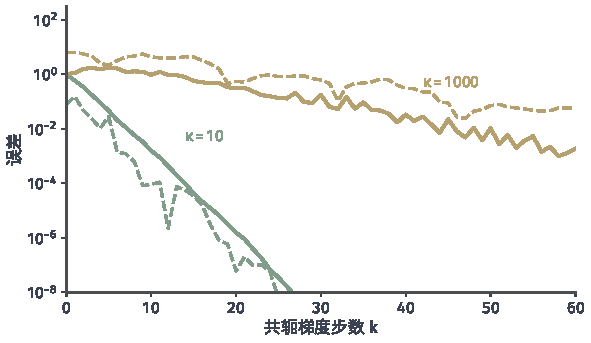
\includegraphics[width=100mm]{figures/05-optimization/07-multiple-criteria-and-nested-optimization/matplotlib/bilevel-cg/figure.pdf}
 \caption{共轭梯度法解伴随方程的收敛，$d=60$，$\bm{H}$的特征值在$[1/\kappa,1]$上对数均匀分布，$\bm{B}$、$\nabla_{\bm{y}}F$是固定种子下的随机单位向量。实线是残差范数，虚线是超梯度的绝对误差。绿色$\kappa=10$，黄色$\kappa=1000$。}
 \label{fig:bilevel-cg}
\end{BookInlineFigure}

\paragraph{另一种近似：Neumann级数}
若$0<\alpha<2/\lambda_{\max}(\bm{H})$，矩阵$\bm{I}-\alpha\bm{H}$的谱半径小于$1$，$\bm{H}^{-1}$可以展开为级数：
\begin{equation}
 \bm{H}^{-1}=\alpha\sum_{k=0}^{\infty}(\bm{I}-\alpha\bm{H})^k.
 \label{eq:bilevel-neumann}
\end{equation}
只取前$\ell$项，就得到一种只用Hessian向量积的近似。它收敛比共轭梯度法慢，但第~\ref{sec:bilevel-truncated}小节会看到，它恰好就是截断展开的极限形式。

\subsection{约束内层}
\label{sec:bilevel-constrained-inner}

内层有约束时，内解满足的不再是驻点方程，$\bm{H}$的位置也要换成整个KKT系统。本小节要解决的问题是：什么时候这样做是对的，以及哪些情况下根本不存在经典的导数。

\paragraph{主要思想：对活动的KKT方程求导}
$g$已用作内层目标，这里把内层约束写成$c_i(\bm{x},\bm{y})\leq0$（$i=1,\ldots,m$）和$h_j(\bm{x},\bm{y})=0$（$j=1,\ldots,p$），Lagrange函数是
\begin{equation}
 \mathcal{L}(\bm{x},\bm{y},\bm{\lambda},\bm{\nu})=g+\sum_{i=1}^{m}\lambda_ic_i+\sum_{j=1}^{p}\nu_jh_j.
 \label{eq:bilevel-lagrangian}
\end{equation}

第~\ref{chap:constrained-optimality}章的KKT条件和第~\ref{chap:parametric-sensitivity}章的敏感性定理告诉我们：在基准KKT点处，若线性无关约束资格（LICQ）、严格互补和二阶充分条件成立，则存在邻域内的连续可微分支，活动集$A$在分支上保持不变，分支上的点都是严格局部极小点。

把活动不等式当成等式，记活动不等式与等式的总数为$a+p$，定义四个矩阵。前两个是$\mathcal{L}$的二阶导数：
\[
 \bm{W}=\nabla^2_{\bm{y}\bm{y}}\mathcal{L},\qquad\bm{B}_{\mathcal{L}}=\nabla^2_{\bm{y}\bm{x}}\mathcal{L}.
\]
另外两个来自约束：$\bm{J}$的行是活动约束和等式约束对$\bm{y}$的梯度，$\bm{E}$的行是它们对$\bm{x}$的梯度。KKT矩阵为
\begin{equation}
 \bm{K}=\begin{bmatrix}\bm{W}&\bm{J}^{\top}\\\bm{J}&\bm{0}\end{bmatrix}.
 \label{eq:bilevel-kkt-matrix}
\end{equation}

\begin{theorem}[约束内层的隐式超梯度]
\label{thm:bilevel-constrained-hypergradient}
设在基准KKT点处$g,c_i,h_j$二阶连续可微，LICQ、严格互补与二阶充分条件成立，$F$连续可微。则$\Phi(\bm{x})=F(\bm{x},\hat{\bm{y}}(\bm{x}))$在基准点附近连续可微，且
\begin{equation}
 \nabla\Phi=\nabla_{\bm{x}}F-\bm{B}_{\mathcal{L}}^{\top}\bm{v}-\bm{E}^{\top}\bm{w},
 \qquad
 \bm{K}\begin{bmatrix}\bm{v}\\\bm{w}\end{bmatrix}=\begin{bmatrix}\nabla_{\bm{y}}F\\\bm{0}\end{bmatrix}.
 \label{eq:bilevel-constrained-hypergradient}
\end{equation}
\end{theorem}

\begin{proof}
由第~\ref{chap:parametric-sensitivity}章的不等式约束解导数定理，$\bm{K}$可逆，分支的Jacobian矩阵$\bm{D}$与乘子导数$\bm{D}_{\bm{w}}$满足
\[
 \bm{K}\begin{bmatrix}\bm{D}\\\bm{D}_{\bm{w}}\end{bmatrix}=-\begin{bmatrix}\bm{B}_{\mathcal{L}}\\\bm{E}\end{bmatrix}.
\]

取$(\bm{v},\bm{w})$为式~\eqref{eq:bilevel-constrained-hypergradient}中方程的解，并用$\bm{K}$对称，得到
\[
 \bm{D}^{\top}\nabla_{\bm{y}}F=\begin{bmatrix}\bm{D}\\\bm{D}_{\bm{w}}\end{bmatrix}^{\top}\bm{K}\begin{bmatrix}\bm{v}\\\bm{w}\end{bmatrix}=-\bm{B}_{\mathcal{L}}^{\top}\bm{v}-\bm{E}^{\top}\bm{w}.
\]
代入第~\ref{sec:bilevel-hypergradient}小节开头的链式法则即得。
\end{proof}

\paragraph{预算例}
外层变量取预算$x=\tau$，内层沿用第~\ref{chap:parametric-sensitivity}章的预算二次问题的主要部分，外层想让配置接近另一个点：
\[
 \begin{aligned}
 g(\bm{y})&=\frac12(y_1-2)^2+\frac12(y_2-1)^2,\quad c(\tau,\bm{y})=y_1+y_2-\tau\leq0,\\
 F(\bm{y})&=\frac12(y_1-2)^2+\frac12(y_2-2)^2.
 \end{aligned}
\]

在$\tau=2$处约束活动，内解和乘子是$\bm{y}=(3/2,1/2)$，$\lambda=1/2>0$，严格互补成立。各块矩阵和右端为
\[
 \bm{W}=\bm{I},\quad\bm{J}=\begin{bmatrix}1&1\end{bmatrix},\quad\bm{B}_{\mathcal{L}}=\bm{0},\quad E=-1,\quad\nabla_{\bm{y}}F=\begin{bmatrix}-1/2\\-3/2\end{bmatrix}.
\]

式~\eqref{eq:bilevel-constrained-hypergradient}的方程组写开是
\[
 v_1+w=-\frac12,\qquad v_2+w=-\frac32,\qquad v_1+v_2=0.
\]

前两式相加并用第三式，得$w=-1$，于是$v_1=1/2$，$v_2=-1/2$。代入超梯度公式，
\[
 \Phi'(2)=-E\,w=-1.
\]

直接核对：约束活动时$\bm{y}=((1+\tau)/2,(\tau-1)/2)$，它对$\tau$的导数是$(1/2,1/2)$，与$\nabla_{\bm{y}}F$的内积是$-1$。图~\ref{fig:bilevel-kkt-kink}(a)的绿线是这条解路径。

\paragraph{公式失效的情形}
活动集变化时导数会断。预算例中$\lambda=(3-\tau)/2$，到$\tau=3$时乘子降为零，严格互补失效，内解停在理想点$(2,1)$。外层值的左导数由$(\tau-4)/2$给出，在$\tau=3$处等于$-1/2$；$\tau>3$时外层值是常数，右导数是$0$。这就是图~\ref{fig:bilevel-kkt-kink}(b)的折点，经典的导数在此不存在。

\begin{BookInlineFigure}
 \centering
 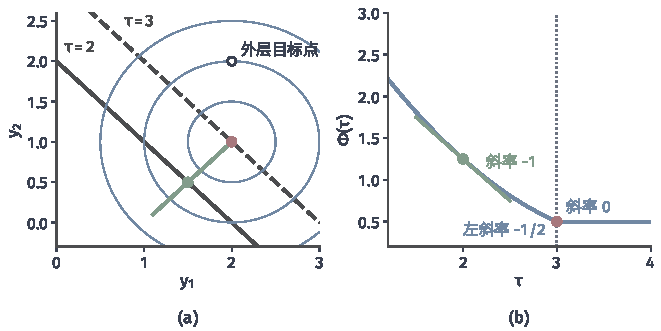
\includegraphics[width=112mm]{figures/05-optimization/07-multiple-criteria-and-nested-optimization/matplotlib/bilevel-kkt-kink/figure.pdf}
 \caption{约束内层的预算例。(a)蓝色等高线属于内层目标，红点是无约束最优$(2,1)$，深灰实线和虚线分别是$\tau=2$和$\tau=3$的预算线，绿线是内解随$\tau$移动的路径，绿点是$\tau=2$的解，空心点是外层目标点$(2,2)$。(b)外层值$\Phi(\tau)$，绿色切线在$\tau=2$处斜率$-1$；红点$\tau=3$处活动集改变，左斜率$-1/2$，右斜率$0$。}
 \label{fig:bilevel-kkt-kink}
\end{BookInlineFigure}

$\bm{K}$奇异时公式不能使用，但内解不一定不可微。取内层$\min\frac12(y-2)^2$，约束$y\leq\tau$和$2y\leq2\tau$是同一条约束的两种写法。在$\tau=1$处两者都活动，$\bm{J}$的两行成比例，LICQ失效，$\bm{K}$奇异，乘子也不唯一。而内解$y=\min\{\tau,2\}$在$\tau=1$附近的导数是$1$，完全正常。

还有一种常见的错误，是把$\bm{H}$换成$\bm{W}$，仍用式~\eqref{eq:bilevel-hypergradient}。预算例中$\bm{W}=\bm{I}$，$\bm{B}_{\mathcal{L}}=\bm{0}$，这样算出的解导数是零向量，而真实导数是$(1/2,1/2)$。约束的作用全在$\bm{J}$和$\bm{E}$里，只换一个矩阵等于把约束的响应丢掉了。
